\section{CLASSE}

A classe é uma estrutura que agrupa as propriedades e os métodos de forma
abstrata com base no modelo de negócio do software que será desenvolvido. 
Sendo assim, é uma estrutura estática que agrupa de maneira lógica e descreve 
propriedades e métodos com base no modelo de negócio representando uma abstração 
da realidade \cite{phpProgramandoComOrientacaoAObjetos}.

Por conta disto, uma classe pode ser considerada como um modelo ou
\textit{template}, no qual, com base nesses modelos podem ser criados vários objetos.

Em uma analogia com o processo de preparação de um bolo, temos a classe como
sendo a receita e o objeto como o bolo. Onde, com base em uma receita podemos fazer 
vários bolos.

Para \citeonline{c++Absoluto}, uma classe é um novo tipo de dados assim como os já
existentes tipos primitivos: \textit{int} e \textit{double}, portanto, um método
ou uma variável podem usar uma classe ao trocarem mensagens, sendo assim a classe 
poderia ser utilizada como dado de entrada ou saída.

Portanto, as classes são os blocos de construção de uma aplicação, que quando
unidos dão origem a um software \cite{learningJava}. Sendo que, pode ser 
composta por: métodos, propriedades, códigos de construção e destruição, 
utilizando conceitos de: herança, polimorfismo, encapsulamento, interfaces e 
exceções. E por fim, um conjunto de classes poderá ser agrupado em um pacote.

\begin{figure}[h!tb]
	\centering
	\caption{Definição de uma Classe na linguagem PHP}
	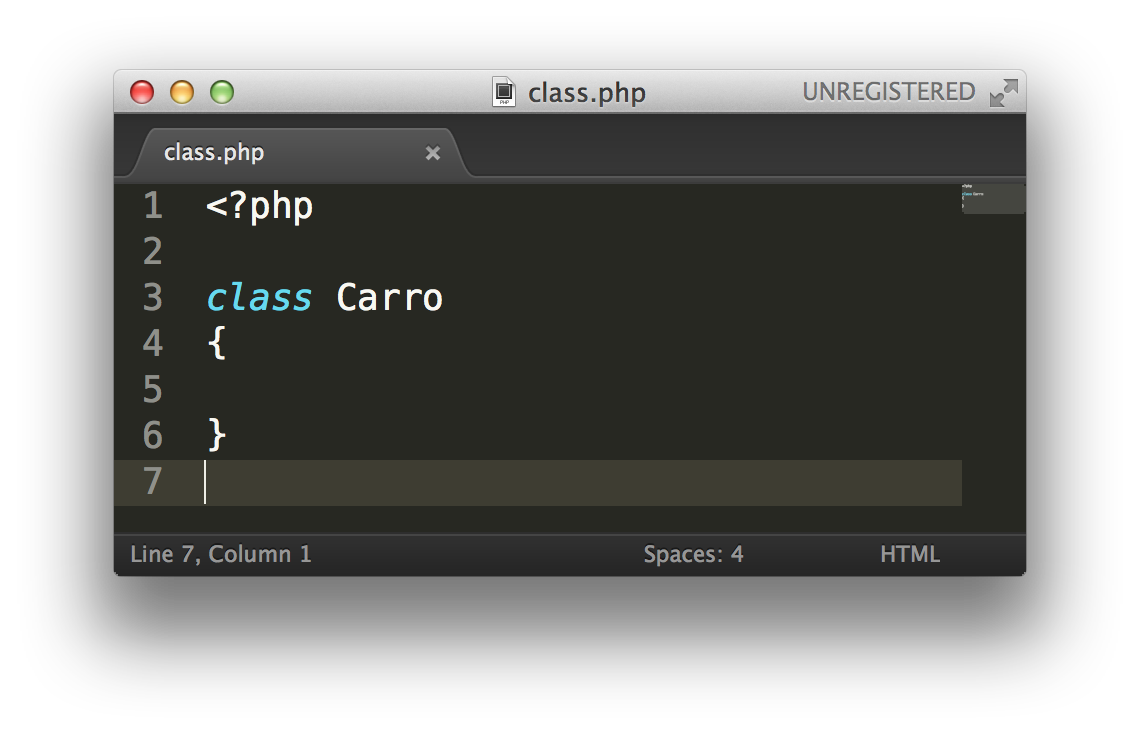
\includegraphics[width=\textwidth]{images/class.png}
	\label{fig:classe}
	\centering
	\footnotesize Fonte: \fonteOAutor
\end{figure}

\FloatBarrier 	% Este comando impede que as imagens 
				% flutuem a partir deste ponto no seu documento

Logo abaixo será apresentada a análise do código exibido na
figura \ref{fig:classe}:

\begin{enumerate}[a)]
    \item \textbf{linha 1:} temos o início da execução de um bloco de código
    PHP;
    \item \textbf{linha 3:} informamos ao interpretador da linguagem PHP que 
    estamos definindo um novo tipo de dados (uma nova estrutura) que será 
    identificada através do nome \textit{Carro};
    \item \textbf{linha 4:} o símbolo \textbf{\{} se refere a abertura de um
    bloco de código, ou seja, informa ao interpretador onde inicia-se a definição de 
    características ou dados (propriedades ou atributos) e ações (métodos). 
    Ambos os conceitos métodos e propriedades veremos ao decorrer deste
    capítulo;
    \item \textbf{linha 6:} o símbolo \textbf{\}} se refere ao fechamento de um
    bloco de código, ou seja, informa ao interpretador onde terminam as
    definições de propriedades e métodos.
\end{enumerate}